\chapter{Experiment Description}
Modern general-purpose detectors used in high-energy colliders typically employ cylindrical detection layers arranged around the beam axis. One such example is the Compact Muon Solenoid (CMS), which is part of the LHC at CERN and is considered one of the largest international scientific collaborations in history. The CMS is designed for a broad physics program that includes studying the Standard Model. This chapter provides a description of the various components of the CMS detector, including the several systems to measure the luminosity with a particular focus on the silicon pixel tracker, which is described in greater detail due to its relevance to the thesis.
 
\section{The Compact Muon Solenoid}

The CMS experiment is one of the four general-purpose detectors situated at the LHC. The CMS detector is constructed around a massive solenoid magnet, which is a cylindrical coil of superconducting cable generating a magnetic field of 4 tesla, this field is used to separate the calorimeter energy deposits of charged and neutral particles in jets. The field is confined by a steel "yoke" which constitutes the bulk of the detector's weight of 14,000 tonnes, the complete detector has a length of 21.6 meters and a diameter of 14.6 meters.  \cite{CMS_Exp_2008}. \\

The CMS detector comprises various detection layers that include separate parts of the detector, these layers are the fine-grained silicon tracker, which provides efficient and precise reconstruction of charged-particle trajectory. The highly-segmented electromagnetic calorimeter (ECAL) wish principal purpose is the detection of  electromagnetic energy and the identification of electrons and photons. The hadronic calorimeter (HCAL) wish principal purpose is the detection of hadrons in jets  \cite{CMS_Exp_2008}. Additionally, there is an excellent muon tracking system. A schematic representation of the CMS detector is shown in Fig. \ref{detector_CMS}.

\begin{center}
  \begin{figure}[ht]
    \centering
    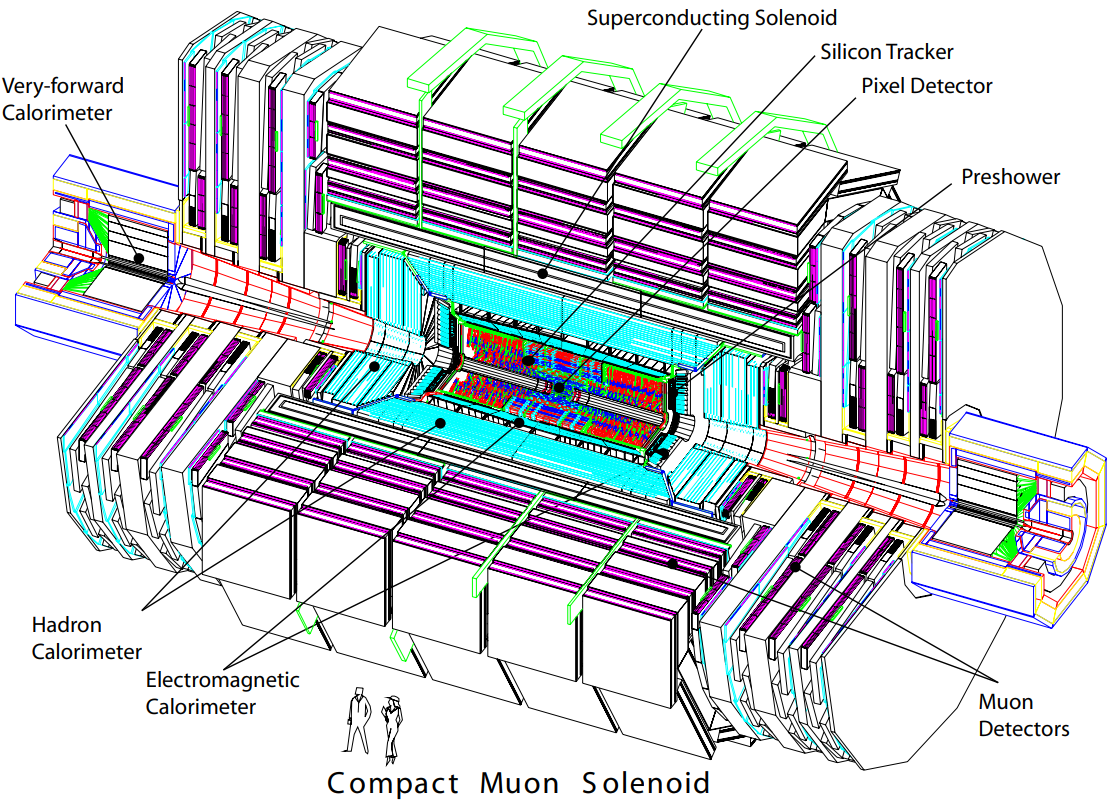
\includegraphics[scale=.3]{Chapter2/CMS_detector_simple.png}
    \caption[Perspective view of the CMS detector]{Perspective view of the CMS detector.}
    \label{detector_CMS}
  \end{figure}
\end{center}

A powerful magnet is required to bend charged particles as they travel outward from the collision point. Bending the trajectory of the particles serves two purposes: first, it helps identify the charge of the particle, as positively and negatively charged particles bend in opposite directions in the same magnetic field; and second, it enables measurement of the particle's momentum.\\

To achieve high precision identification of the paths of deflected charged particles, the CMS employs a silicon tracker as its most inner detector to the beam pipe. This tracker system utilizes silicon strips and pixels that are divided into several layers in order to register the tracks of these particles. As a charged particle passes through a Tracker layer, it interacts electromagnetically with the silicon and produces a hit. By combining these individual hits, the track of the traversing particle can be identified \cite{CMS_Exp_2008}. Further details about the tracker system can be found in the next section.\\

ECAL measures the energy of electrons and photons by completely stopping them. It is a hermetic, homogeneous calorimeter consisting of 61,200 lead tungstate (PbWO4) crystals mounted in the central barrel part and closed by 7,324 crystals in each of the two endcaps. In front of the endcap crystals, a preshower detector is placed. Avalanche photodiodes (APDs) are used as photodetectors in the barrel and vacuum phototriodes (VPTs) in the endcaps.\\ 

The HCAL surrounds the ECAL and together they complete a hermetic calorimetry system designed to measure jets and missing transverse energy. When hadrons, which are composite particles consisting of quarks and gluons, travel through the ECAL, they are stopped by the HCAL, to achieve  this, the HCAL is divided into four parts: the hadron barrel (HB), hadron outer (HO), hadron endcap (HE), and hadron forward \cite{det_summary}.\\

The final particle that the CMS directly observes is the muon. Muons are approximately 200 times heavier than electrons and are not stopped by the calorimeters. Therefore, special sub-detectors have to be constructed to detect them as they traverse the CMS. These sub-detectors are interleaved with the return yoke of the solenoid. The large magnet of the CMS also allows us to measure each muon's momentum both inside the superconducting coil (using the tracking devices) and outside of it (using the muon chambers) \cite{det_summary}. 

A transverse slice of the CMS detector, depicting specific particle interactions, is shown in Figure \ref{slice_CMS}.


\begin{center}
  \begin{figure}[ht]
    \centering
    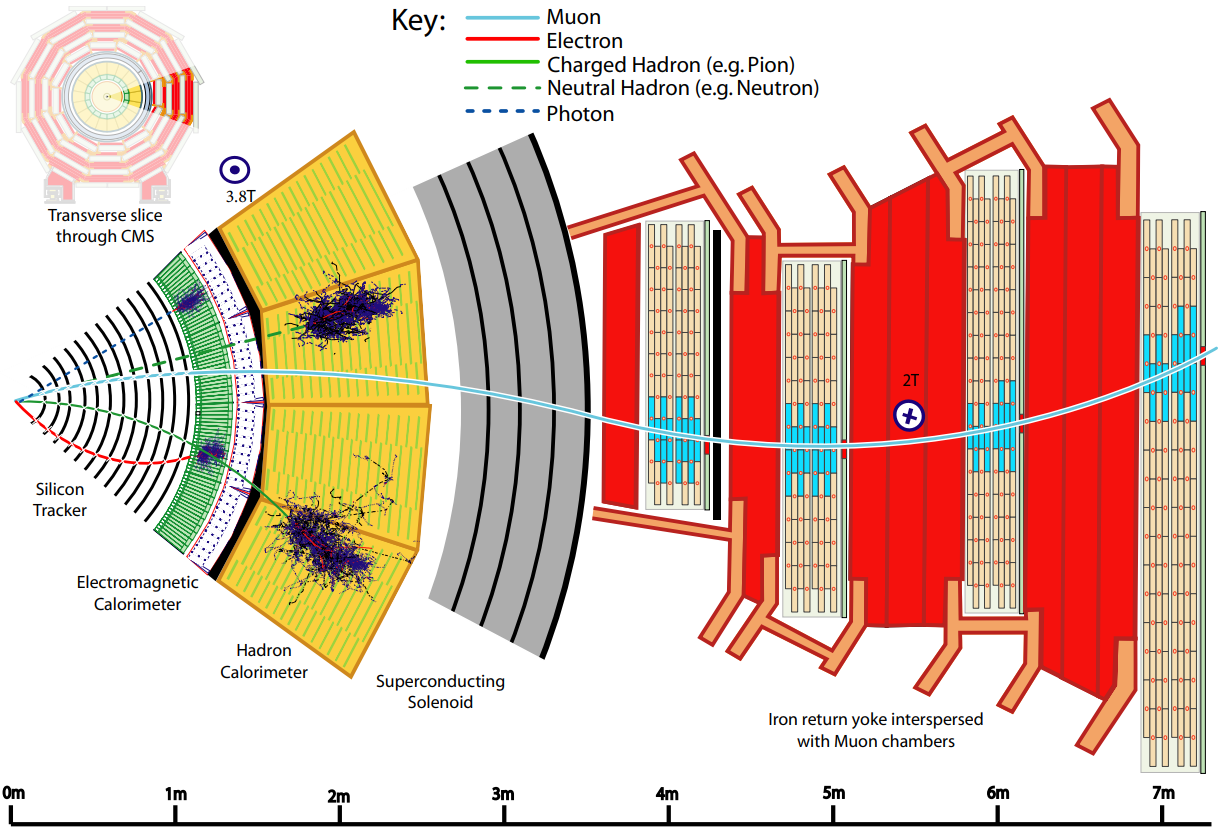
\includegraphics[scale=.3]{Chapter2/slice_det.png}
    \caption[Transverse slice view of the CMS detector]{Transverse slice of the CMS detector with some particle interactions (from the beam interaction region to the muon detector) \cite{det_summary}.}
    \label{slice_CMS}
  \end{figure}
\end{center}

The CMS's coordinate system has its origin located at the center of the detector, with the $y$-axis oriented vertically upwards and the $x$-axis directed radially inward, toward the center of the LHC. As a result, the z-axis aligns with the direction of the beam. In this system, the azimuthal angle $\varphi$ is measured from the $x$-axis within the $x-y$ plane, while the radial coordinate in this plane is represented by $r$. Furthermore, the polar angle $\theta$ is measured with respect to the z-axis, seudorapidity is defined as $\eta = − ln tan(\theta/2)$ \cite{CMS_Exp_2008}.

\section{CMS Luminometers}

A total of seven systems are used for measuring luminosity at CMS. The Pixel Luminosity Telescope (PLT) and Fast Beam Conditions Monitor (BCM1F) are dedicated systems for luminosity measurement, while the hadronic forward calorimeter (HF) uses a dedicated readout on an existing system. Additionally, three other methods, the drift tube luminosity (DT), the pixel cluster counting method (PCC), and the vertex counting method (VTX), use data from existing parts of the CMS detector to perform a luminosity measurement using the main CMS DAQ system. The PCC measurement uses the data collected with the standard CMS trigger system with triggers requiring colliding bunches but not any specific event activity, known as "zero-bias" triggers. Finally, the RAMSES detectors are part of the LHC environmental protection and monitoring systems, but they can also be used to provide a luminosity measurement readout through Timber (operational data and LHC logging service) \cite{pas_18}.  A brief overview of the CMS luminometers is provided below.\\

PLT Is a dedicated system for measuring luminosity using silicon pixel sensors. There are a total of 48 sensors arranged into 16 “telescopes”, eight at either end of CMS outside the pixel endcap, where each telescope contains three sensor planes arranged nearly parallel to the beam pipe. The PLT measures the rate of “triple coincidences”, where a hit is observed in all three planes, typically corresponding to a track from a particle originating at the interaction point. The overall mean rate for PLT  is estimated using the zero-counting method, where it is assumed that the number of observed triple coincidences follows a Poisson distribution \cite{pas_18}. \\

BCM1F for Run 2 comprised a total of 24 sensors mounted on the same carriage as the PLT, consisting of 10 silicon sensors, 10 polycrystalline diamond (pCVD) sensors, and 4 single-crystal diamond (sCVD) sensors. The BCM1F readout features a fast readout with 6.25 ns time resolution; the precise time measurement, in conjunction with the position of BCM1F at 1.8 m from the center of CMS, allows hits from collision products to be separated from hits from machine-induced background, because the incoming background is separated in time from the outgoing collision products  \cite{pas_18}.\\ 

HF luminosity measurement uses a dedicated readout system installed in the HF ccalorimeter readout electronics. Only two HF rings are used for luminosity measurement to ensure relatively uniform occupancy. Two algorithms are available: the first relies on the fraction of occupied towers (HFOC), and the second is based on the sum of the transverse energy ET (HFET)  \cite{pas_18}.\\

DT luminosity measurement uses the rate of muon track stubs in the muon barrel track finder. The DT algorithm used does not provide bunch-by-bunch measurements and is thus applicable only for the total luminosity measurement. DT measurement is generally  stable and linea so it provides a complementary offline reference measurement. The rate in DT during VdM fills is too low to allow for calibration using the vdM scan, so it is cross-calibrated to another detector \cite{pas_18}.\\

RAMSES  is a CERN radiation and environmental monitoring sytem. Althoug is not designed as a luminometer, the rate observed in this detector does function quite well as a luminosity measurement. The sensor itself is a cylindrical plastic ionization chamber filled with 3 L of air at atmospheric ressure and it primarily detects photons.  The overall rate is small, which means that it is not capable of making bunch by bunch measurements and cannot be independently calibrated using a vdM scan; however, this also means it is less affected by issues such as instability caused by radiation damage or nonlinearity \cite{pas_18}.\\

The PCC method uses the rate of pixel clusters in the CMS pixel detector to provide a luminosity measurement this method will be described in more detail in chapter 3.  

The location of the 7 luminometers in the CMS experiment are shown in Figure \ref{luminometers}.

\begin{center}
  \begin{figure}[ht]
    \centering
    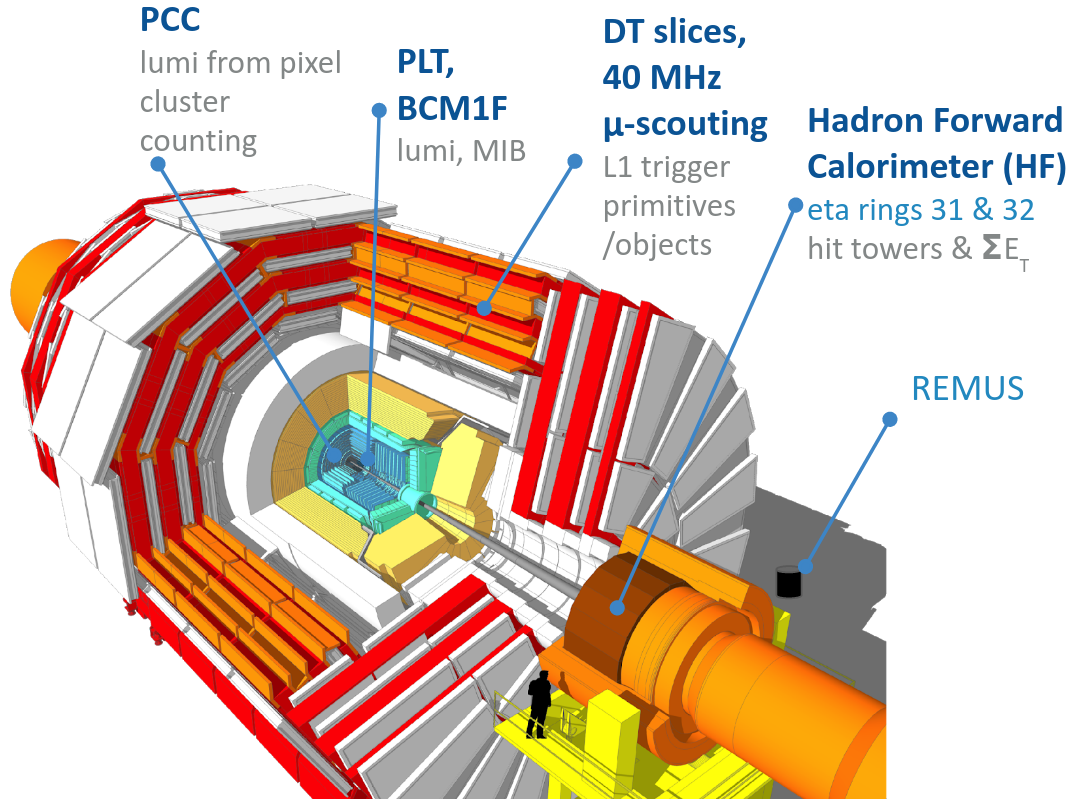
\includegraphics[scale=.3]{Chapter2/detectors.png}
    \caption[Layout of the luminometers in the CMS detector]{The seven luminometers that make up the CMS luminosity measurement system. Multiple independent systems used online: BCM1F, HFET, HFOC, PLT (independently calibrated) ,REMUS and  DT (cross-calibrated) , Pixel cluster counting is used after offline processing.}
    \label{luminometers}
  \end{figure}
\end{center}

\section{CMS Tracking System}

The tracking system plays a crucial role in precisely measuring the trajectories and momenta of charged particles generated by collisions in the LHC, as well as reconstructing secondary vertices. It has a total physical size of 5.8 m in length and 2.5 m in diameter. 
The CMS tracking detector relies on semiconductor technology, this is divided in two systems, the pixel detector and the Strip tracker \cite{CMS_Exp_2008}. In Figure \ref{strip_layout}, we can observe the pixel detector at the center, surrounded by the Strip tracker.\\

The Strip tracker is comprised of two subsystems: the first being the Tracker Inner Barrel (TIB) and Disks (TID), which is further divided into four barrel layers and three disks at each endcap. The second subsystem is the Tracker Outer Barrel (TOB), which consists of six barrel layers and the Tracker EndCaps (TEC) comprising of nine disks. The Strip tracker in total comprises of 15148 silicon modules, covering an active area of about 198$\text{m}^{2}$, and consists of 9.3 million strips \cite{CMS_Exp_2008}. \\

The innermost part of the tracking system is made up of the silicon pixel tracker, which consists of four concentric barrel layers (BPIX) and three disks on each endcap (FPIX). This component comprises a total of 70 million pixels and extends the tracker's acceptance up to a pseudorapidity of $|\eta| < 2.5$. More information about this detector is provided in the following section.

\begin{center}
  \begin{figure}[ht]
    \centering
    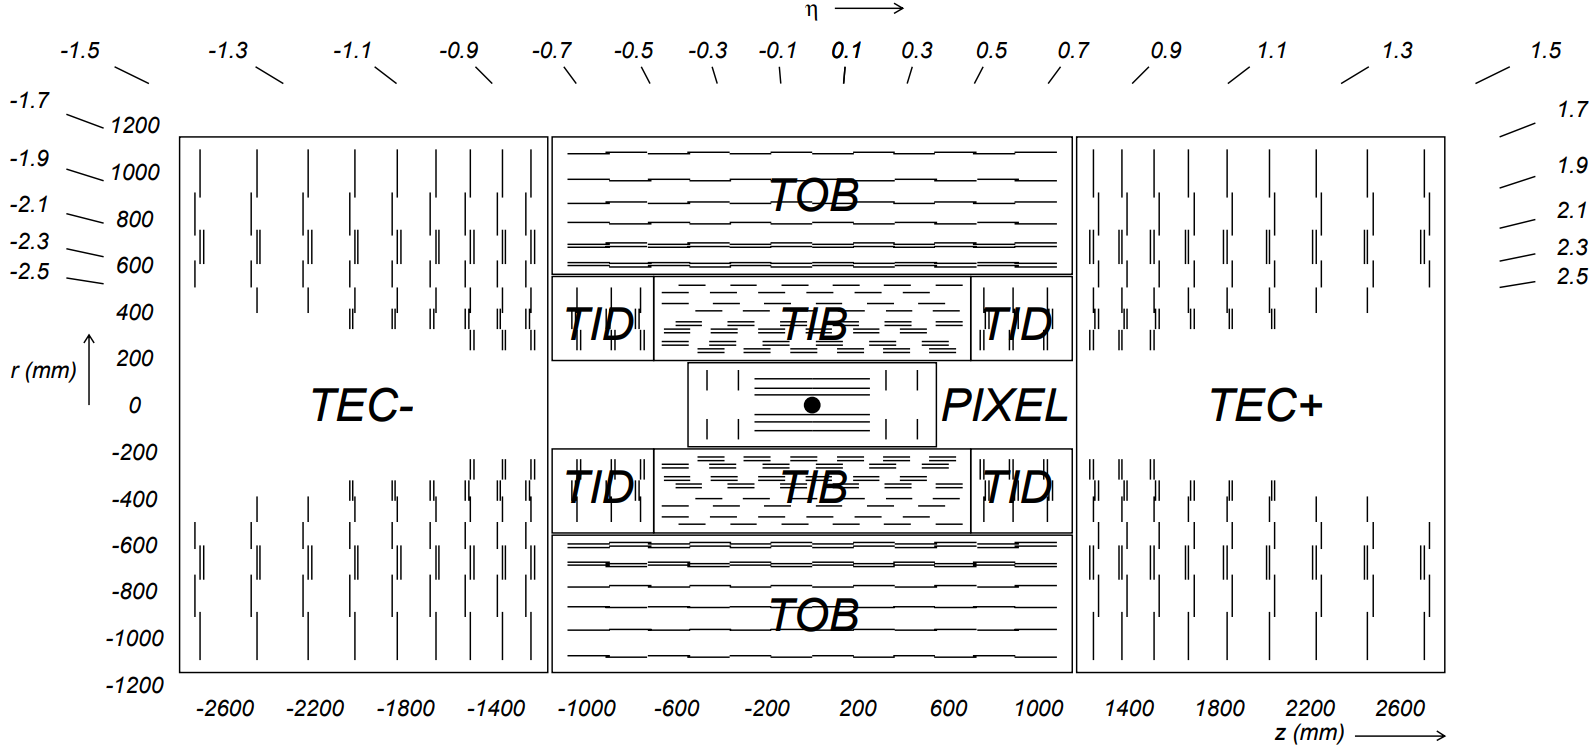
\includegraphics[scale=.23]{Chapter2/strip_layout.png}
    \caption[Schematic cross section through the CMS tracker]{Schematic cross section through the CMS tracker \cite{CMS_Exp_2008}.}
    \label{strip_layout}
  \end{figure}
\end{center}


\section{Silicon Pixel Detector}

The silicon pixel detector  forms the innermost component of the tracking system. This detector facilitates the provides complete spatial coverage over the area nearest to the interaction point, which, in turn, enables precise tracking of charged particles and vertex reconstruction. The coverage of the pixel detector is in the pseudorapidity range $(|\eta| < 2.5)$, operating in a radiation rich environment, marked by high track density \cite{phase1_Pixel_Detector}.\\

The CMS pixel detector encompasses four concentric barrel layers (L1-L4), each with radii measuring 29, 68, 109, and 160 mm, and three disks (D1-D3) on either end positioned at distances of 291, 396, and 516 mm from the detector's center. The complete detector is built from 1856 segmented silicon sensor modules.\\  

A schematic of the CMS Phase-1 pixel detector's arrangement is depicted in Figure \ref{phase1_pixel_detector} where the total silicon area spans 1.9 $\text{m}^{2}$, here The BPIX and FPIX detectors are equipped with four service half-cylinders each, with a combined length of 540 mm. These cylinders host the readout and control circuits, and provide guidance for the power lines and cooling tubes of the detector.
\begin{center}
  \begin{figure}[h]
    \centering
    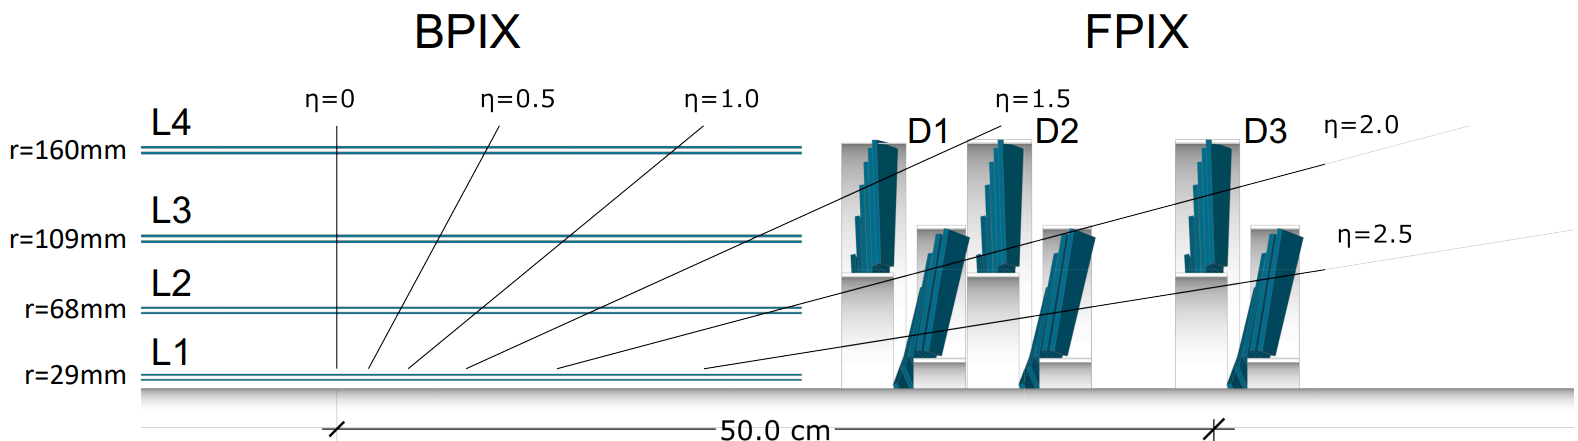
\includegraphics[scale=.26]{Chapter2/phase1_PixelDetector.png}
    \caption[CMS Phase-1 pixel detector]{Layout of the CMS Phase-1 pixel detector in longitudinal view\cite{phase1_Pixel_Detector}.}
    \label{phase1_pixel_detector}
  \end{figure}
\end{center}

 
The BPIX detector is bifurcated into two mechanically self-sufficient halves, both of which are made up of a half detector and two service half-cylinders. BPIX is built in total from 1184 segmented silicon sensor modules where the orientation of their surface  in both halves is parallel to the magnetic field.\\

On the other hand, the FPIX detector is segmented into four mechanically independent quadrants, each of which comprises three half-disks housed in a service half-cylinder. The sensor orientation in the FPIX detector is arranged such that the long side of the pixel is aligned with the radial direction. FPIX is built in total from 672 segmented silicon sensor modules and the half-disks are additionally subdivided into inner and outer half-rings that support 22 and 34 modules, respectively \cite{phase1_Pixel_Detector}.\\

A pixel detector module is built from a planar silicon sensor with a size of 18.6 $\times$ 66.6 $\text{mm}^{2}$ (active area of 16.2 $\times$ 64.8 $\text{mm}^{2}$). Each module consists of a sensor with 160$\times$416 pixels  bump-bonded to an array of 2$\times$8 readout chips (ROC's). Each ROC is segmented into 4160 readout channels and reads out the pulse height information for each pixel, in total there are 124 million readout channels. The standard pixel size is 100$\times$150 $\mu m^{2}$\\

Figure \ref{modules_drawing} illustrates the modules of the CMS Phase-1 pixel detector \cite{phase1_Pixel_Detector}, while Figure \ref{module and hit} on the left depicts the layout of the silicon sensor connected to the readout chip. On the right side of Figure \ref{module and hit}, a charged particle can be seen passing through a pixel, providing enough energy to eject electrons from the silicon atoms. A voltage applied to the sensor allows the collection of these charges as a small electric signal, which is then amplified by an electronic readout chip.

\begin{center}
  \begin{figure}[h]
    \centering
    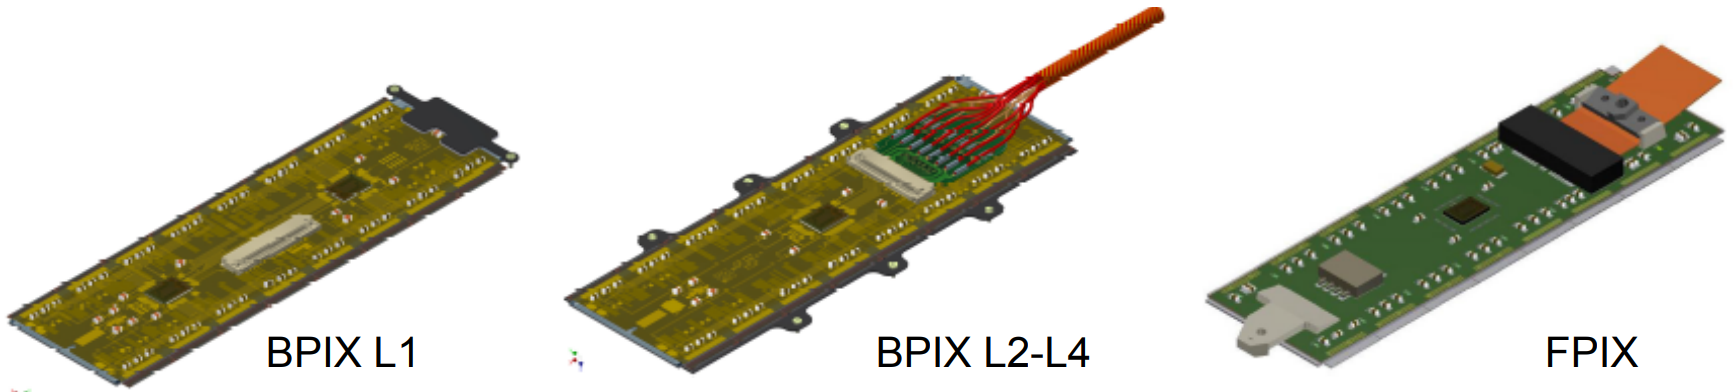
\includegraphics[scale=.2]{Chapter2/modules_drawing.png}
    \caption[Types of modules in the pixel detector]{ Drawings of the pixel detector modules for BPIX L1 (left), BPIX L2–4 (middle), and the FPIX detector (right)\cite{phase1_Pixel_Detector}.}
    \label{modules_drawing}
  \end{figure}
\end{center}

\begin{center}
  \begin{figure}[h]
    \centering
    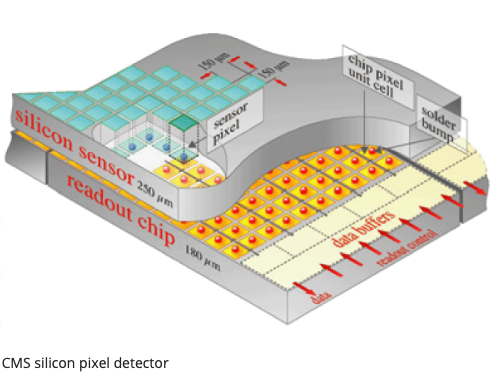
\includegraphics[scale=.3]{Chapter2/PixelSensor.png} 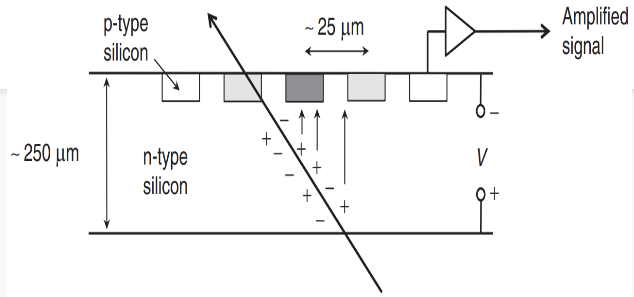
\includegraphics[scale=.3]{Chapter2/hit.png}
    \caption[Schematic view of a pixel sensor and its connection to the readout channels]{ left: layout pixel sensor conected to a readout chip , right: hits detection in a corresponding  pixel sensor \citep{thomson_2013}. }
    \label{module and hit}
  \end{figure}
\end{center}

\section{Pixel Cluster Reconstruction}

The track reconstruction process involves several steps. Firstly, zero-suppressed signals above specified thresholds in pixel  channels  are used to form clusters. The charge measured within each cluster corresponds to the charge deposited by a single charged particle. Next, the cluster positions and their uncertainties are estimated in a local orthogonal coordinate system  in the plane of each sensor \cite{Track_Reco_2014}. \\

To be considered a valid cluster, each one must have a minimum charge equivalent to 4000 electrons \cite{Track_Reco_2014,phase1_Pixel_Detector}. For normally incident minimum-ionizing particles (MIPs) in a silicon sensor with a thickness of 285 $\mu \text{m}$, the most probable value of energy deposition corresponds to approximately 21,000 electrons. However, this charge is often spread over more than one pixel due to Lorentz drift,  which causes the electrons to be pushed due to the force generated by the electromagnetic field, leading to charge clusters.\\

Figure \ref{cluster}  shown an example of how a pixel cluster is constructed. Each square in the figure represents a pixel. The red pixels indicate that they have the required charge up to 2000 electrons to be considered valid pixels and are therefore included in the cluster. On the other hand, the green pixels correspond to charge depositions below the 2000 electron threshold and are not included in the cluster.
The dotted blue line in the figure represents the trajectory of the particle traveling parallel to the x-z plane. As it travels, it activates pixels in its path precisely, as well as pixels that are deviated from its trajectory due to the Lorentz drift \cite{Pixel_Hit_Reconstruction}.\\
\newpage
\begin{center}
  \begin{figure}[h]
    \centering
    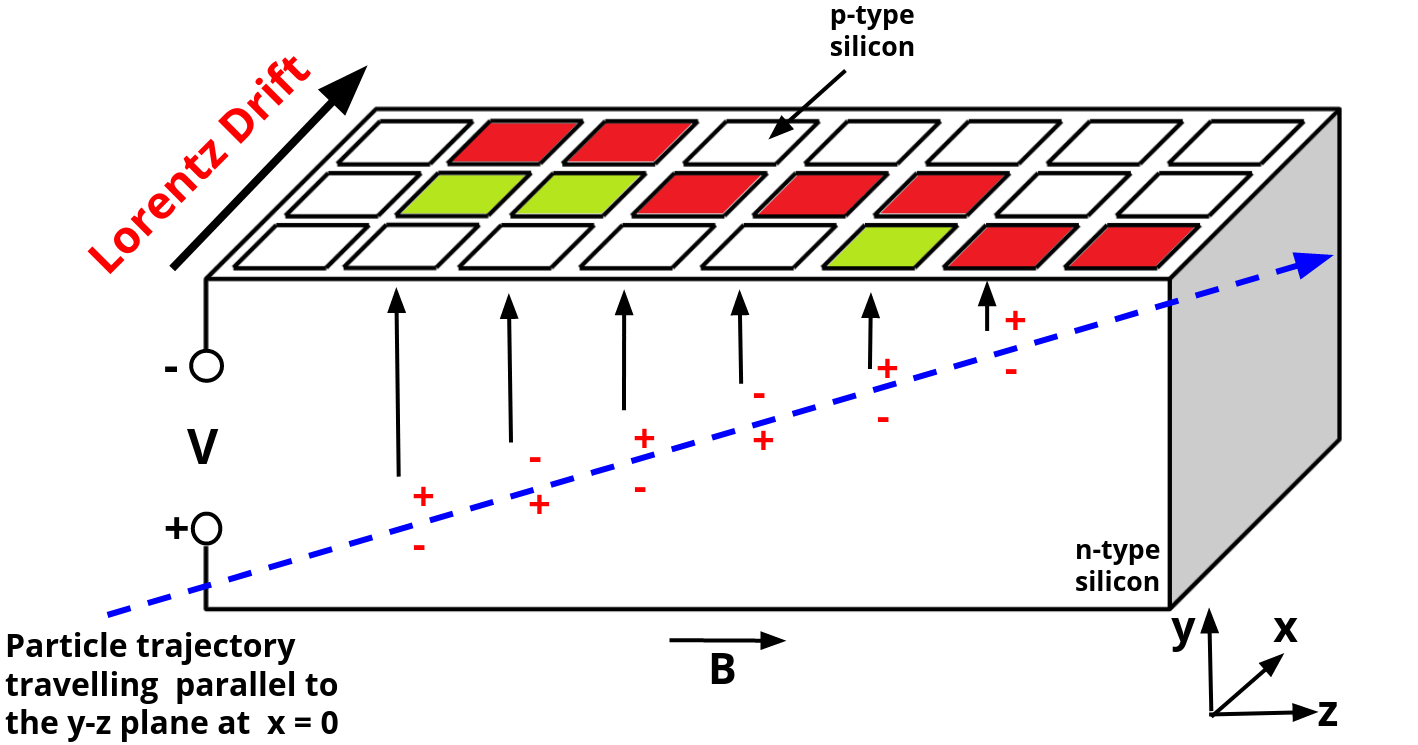
\includegraphics[scale=.25]{Chapter2/pixel_cluster.png} 
    \caption[Construction of a pixel cluster]{ The figure illustrates a pixel cluster example with a total charge up of 4,000 electrons, required to be a valid cluster. The red pixels have the required charge while the green one does not.}
    \label{cluster}
  \end{figure}
\end{center}
